\documentclass{beamer}

\usepackage{minted}
\usemintedstyle{eclipse}

\useoutertheme{infolines}
\setbeamertemplate{headline}{}
\setbeamertemplate{footline}{
  \hfill
  \usebeamercolor[fg]{page number in head/foot}
  \usebeamerfont{page number in head/foot}
  \insertpagenumber\kern1em\vskip10pt
}
\setbeamertemplate{navigation symbols}{}

\usepackage{tikz}
\usetikzlibrary{arrows}

\title{Lightweight Functional Logic Meta-Programming}
\subtitle{in Scala}
\author{Nada Amin, Tiark Rompf}
\institute{LAMP, EPFL}
\date{March 4, 2014}

\begin{document}

\frame{\titlepage}

\begin{frame}[fragile]{Logic Programming (Prolog)}
\begin{columns}
\begin{column}[t]{8cm}
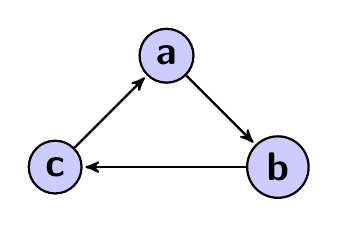
\begin{tikzpicture}[->,>=stealth',shorten >=1pt,auto,node distance=2cm,
  thick,main node/.style={circle,fill=blue!20,draw,font=\sffamily\Large\bfseries}]

  \node[main node] (1) {a};
  \node[main node] (2) [below right of=1] {b};
  \node[main node] (3) [below left of=1] {c};

  \path[every node/.style={font=\sffamily\small}]
    (1) edge node [right] {} (2)
    (2) edge node [right] {} (3)
    (3) edge node [right] {} (1);

\end{tikzpicture}
\begin{minted}{prolog}
edge(a,b).
edge(b,c).
edge(c,a).

path(X, Y) :- edge(X, Y).
path(X, Z) :- edge(X, Y), path(Y, Z).
\end{minted}
\end{column}
\begin{column}[t]{4cm}
\begin{minted}{prolog}
?- edge(a, X).
X = b.

?- edge(X, a).
X = c.

?- path(a, X).
X = b ;
X = c ;
X = a ;
X = b .
\end{minted}
\end{column}
\end{columns}
\end{frame}

\begin{frame}[fragile]{Logic Programming (Scala)}
\begin{minted}{scala}
def edge(x: Exp[String], y: Exp[String]): Rel =
  (x === "a") && (y === "b") ||
  (x === "b") && (y === "c") ||
  (x === "c") && (y === "a")

def path(x: Exp[T], y: Exp[T]): Rel =
  edge(x,y) ||
  exists[T] { z => edge(x,z) && path(y,b) }

// Queries
run[(String,String)] { case Pair(x,y) => edge(x,y) }
//=> pair(a,b), pair(b,c), pair(c,a)

runN[String](10) { q => path("a",q) }
//=> b, c, a, b, c, a, b, c, a, b
\end{minted}
\end{frame}

\begin{frame}[fragile]{Deep Linguistic Reuse: OO Encapsulation}
\begin{minted}{scala}
trait Graph[T] {
  def edge(x: Exp[T], y: Exp[T]): Rel
  def path(x: Exp[T], y: Exp[T]): Rel =
    edge(x,y) ||
    exists[T] { z => edge(x,z) && path(y,b) }
}
val g = new Graph[String] {
  def edge(x:Exp[String],y:Exp[String]) =
    (x === "a") && (y === "b") ||
    (x === "b") && (y === "c") ||
    (x === "c") && (y === "a")
}
\end{minted}
\end{frame}

\begin{frame}[fragile]{Deep Linguistic Reuse: Type Classes}
\begin{minted}{scala}
trait Ord[T] { def lt(x:Exp[T],y:Exp[T]): Rel }

implicit class OrdOps[T:Ord](x:Exp[T]) {
  def <(y:Exp[T]): Rel =
    implicitly[Ord[T]].lt(x,y)
}

implicit val ordNat = new Ord[Int] {
  def lt(x:Exp[Int],y:Exp[Int]): Rel =
    // ... elided
}


run[Int] { q => q < 4 } //=> 0,1,2,3
\end{minted}
\end{frame}

\begin{frame}[fragile]{Type Classes: Lexicographic Ordering on Polymorphic Lists}
\begin{minted}{scala}
implicit def ordList[T:Ord] = new Ord[List[T]] {
  def lt(as:Exp[List[T]],bs:Exp[List[T]]): Rel = 
    exists[T,List[T]] { (b,bs1) => 
      (bs === cons(b,bs1)) && {
      (as === nil) || exists[T,List[T]] { (a,as1) =>
      (as === cons(a,as1)) && {
      (a < b) || (a === b) && (as1 < bs1) }}}}

run[List[Int]] { q => q < List(0,1,2) }
//=> nil
//   cons(z,nil)
//   cons(z,cons(z,x0))
//   cons(z,cons(s(z),nil)),
//   cons(z,cons(s(z),cons(z,x0)))
//   cons(z,cons(s(z),cons(s(z),x0)))
\end{minted}
\end{frame}

\begin{frame}[fragile]{Type Classes: Run Queries Forwards and Backwards}
\begin{minted}{scala}
run[String] { q =>
  val t = tree(List(1,1,1) -> "a",
               List(1,2,2) -> "b",
               List(2,1,1) -> "c")
  lookup(t,List(1,2,2),q)
} //=> b
run[Int] { q =>
  val t = tree(List(1,1,1) -> "a",
               cons(q,List(2,2)) -> "b",
               List(2,2,2) -> "c")
  lookup(t,List(1,2,2),"b")
} //=> 1
\end{minted}
\end{frame}

\begin{frame}[fragile]{Vanilla Meta-Interpreter (Prolog)}
\begin{minted}{prolog}
/*
  A meta-interpreter for pure Prolog (Art of Prolog, 17.5)

  solve(Goal) :-
     Goal is true given the pure Prolog program defined by clause/2.
*/

     solve(true).
     solve((A,B)) :- solve(A), solve(B).
     solve(A) :- clause(A,B), solve(B).
\end{minted}
\end{frame}
\end{document}
